% Worked instance of the executable paper template.
% Contract: ../references/paper-writing-template.md
\documentclass{article}
\PassOptionsToPackage{numbers,compress}{natbib}
\usepackage[final]{neurips_2025}
% Executable visual system distilled from arXiv:2506.21656.
% Keep the NeurIPS geometry unchanged. Replace content, not the page grammar.
% Contract: ../references/paper-writing-template.md

% ---------------------------------------------------------------- packages
\usepackage[T1]{fontenc}
\usepackage{microtype}
\usepackage{amsmath,amssymb,amsfonts}
\usepackage{bm}
\usepackage{nicefrac}
\usepackage{booktabs}
\usepackage{graphicx}
\usepackage{array}
\usepackage{ragged2e}
\usepackage{enumitem}
\usepackage{multirow}
\usepackage{makecell}
\usepackage{pifont}
\usepackage{xspace}
\usepackage{adjustbox}
\usepackage{wrapfig}
\usepackage{tabularx}
\usepackage{threeparttable}
\usepackage{siunitx}
% xcolor must be loaded with its options BEFORE colortbl and nicematrix,
% otherwise nicematrix pulls in an option-free xcolor and the build dies with
% "Option clash for package xcolor".
\usepackage[table,dvipsnames]{xcolor}
\usepackage{colortbl}
\usepackage{nicematrix}
\usepackage{tikz}
\usetikzlibrary{arrows.meta,backgrounds,calc,fit,positioning,shapes.geometric}
\usepackage{pgfplots}
\usepgfplotslibrary{fillbetween}
\pgfplotsset{compat=1.18}
\usepackage{subcaption}
\usepackage[most]{tcolorbox}
\usepackage[colorlinks=true,linkcolor=ACBlue,citecolor=ACBlue,urlcolor=ACBlue]{hyperref}
\usepackage[nameinlink,capitalize,noabbrev]{cleveref}

% ------------------------------------------------------------------ palette
% Semantic families. Color is a redundant grouping cue, never the encoding.
\definecolor{ACBlue}{HTML}{1A4E8A}      % primary
\definecolor{ACCyan}{HTML}{56BBCC}      % secondary
\definecolor{ACLink}{HTML}{9A36FF}      % project link only
\definecolor{ACNeutral}{RGB}{230,230,230}   % neutral / reference family
\definecolor{ACCompare}{RGB}{252,228,214}   % comparison family
\definecolor{ACPrimary}{RGB}{207,234,242}   % this study's family
\definecolor{ACInk}{HTML}{15243A}
\definecolor{ACMuted}{HTML}{65758B}
\definecolor{ACGreen}{HTML}{2E8B57}

% -------------------------------------------------------- slot enforcement
% \slot{...} marks a value that evidence must supply.
%   draft build      -> grey bracketed marker, compiles
%   --final build    -> hard LaTeX error, build fails
% This is the mechanical guarantee that no placeholder reaches a submission.
\newif\ifACfinal\ACfinalfalse
\newcommand{\slot}[1]{%
  \ifACfinal
    \PackageError{acpaper}{Unfilled slot: #1}%
      {Every \string\slot\space must be replaced with verified evidence before a
       final build. See references/paper-writing-template.md section 9.}%
  \else
    \textcolor{ACMuted}{\textit{[#1]}}%
  \fi
}

% ------------------------------------------------------------- text macros
\newcommand{\ie}{\textit{i.e.},\xspace}
\newcommand{\eg}{\textit{e.g.},\xspace}
\newcommand{\wo}{\textit{w/o}\xspace}
\newcommand{\cmark}{\textcolor{ACGreen}{\ding{51}}}
\newcommand{\xmark}{\textcolor{BrickRed}{\ding{55}}}
\newcommand{\best}[1]{\textbf{#1}}
\newcommand{\second}[1]{\underline{#1}}
\newcommand{\up}{$\uparrow$}
\newcommand{\down}{$\downarrow$}

% Inline swatch used to introduce a table's row-tint families in prose.
\newcommand{\tightcolorbox}[2]{%
  \begingroup\setlength{\fboxsep}{1pt}\colorbox{#1}{#2}\endgroup
}
% Caption-legend swatch, matching the exemplar's caption key.
\newcommand{\swatch}[1]{\colorbox{#1}{\phantom{\rule{1ex}{1ex}}}}

% ------------------------------------------------------- reference formats
\crefname{equation}{Eq.}{Eqs.}
\crefformat{section}{\S#2#1#3}
\crefformat{subsection}{\S#2#1#3}
\crefformat{subsubsection}{\S#2#1#3}
\crefrangeformat{section}{\S\S#3#1#4 to~#5#2#6}
\crefmultiformat{section}{\S\S#2#1#3}{ and~#2#1#3}{, #2#1#3}{ and~#2#1#3}

% ----------------------------------------------------------- title system
% Page-1 mark, drawn in TikZ so the front page needs no external asset.
% Never reuse the exemplar's logo.
\newcommand{\ProjectMark}{%
  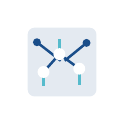
\begin{tikzpicture}[baseline=-0.75ex,scale=0.84]
    \fill[ACBlue!12,rounded corners=2.5pt] (-0.52,-0.52) rectangle (0.52,0.52);
    \draw[ACBlue,line width=0.9pt] (-0.28,-0.15) -- (-0.04,0.12) -- (0.26,-0.10);
    \draw[ACCyan,line width=1.1pt] (-0.28,-0.15) -- (-0.28,-0.36);
    \draw[ACCyan,line width=1.1pt] (-0.04,0.12) -- (-0.04,0.35);
    \draw[ACCyan,line width=1.1pt] (0.26,-0.10) -- (0.26,-0.34);
    \draw[ACBlue,line width=0.9pt] (-0.38,0.30) -- (-0.02,0.02);
    \draw[ACBlue,line width=0.9pt] (0.04,0.02) -- (0.37,0.29);
    \fill[white] (-0.28,-0.15) circle (0.09);
    \fill[white] (-0.04,0.12) circle (0.09);
    \fill[white] (0.26,-0.10) circle (0.09);
    \fill[ACBlue] (-0.38,0.30) circle (0.06);
    \fill[ACBlue] (0.37,0.29) circle (0.06);
  \end{tikzpicture}%
}

\newcommand{\TitleBlock}[1]{%
  \vspace{-0.2cm}
  \begin{tabular}{@{}m{1.32cm}m{12.10cm}@{}}
    \centering\ProjectMark &
    \begin{tabular}[t]{@{}l@{}}
      #1
    \end{tabular}
  \end{tabular}%
}

% neurips_2025.sty renders \@author inside a plain `tabular[t]{c}` cell, whose
% `c` column has no width constraint: it sizes to the content's natural width
% and only centers it, so a normal-length affiliation line (institution name,
% \qquad, second institution) overflows the text block symmetrically on both
% sides. This is independent of the title, and independent of author-name
% length. Fixing it means bounding the content's own width before the style
% file ever sees it: wrap \author{...} in this, and the outer `c` column
% takes on the minipage's fixed, safe width and wraps long lines instead.
\newcommand{\AuthorBlock}[1]{%
  \begin{minipage}{0.92\textwidth}
    \centering
    #1
  \end{minipage}%
}

% ------------------------------------------------------------ tikz styles
% Tier C structural diagrams (references/figure-ladder.md).
\tikzset{
  acbox/.style={rounded corners=2.5pt,draw=ACBlue!55,line width=0.7pt,fill=white,inner sep=4pt},
  acsoft/.style={rounded corners=2.5pt,draw=ACCyan!65,line width=0.7pt,fill=ACPrimary!35,inner sep=4pt},
  acarrow/.style={-{Latex[length=2.2mm]},line width=0.8pt,draw=ACBlue!80},
  acnote/.style={font=\scriptsize,text=ACMuted,align=center}
}

% Tier B plot defaults, so every pgfplots figure shares one visual key.
\pgfplotsset{
  acplot/.style={
    width=0.92\linewidth, height=5.0cm,
    ymajorgrids, grid style={ACMuted!25,line width=0.4pt},
    axis line style={ACInk!70},
    tick label style={font=\scriptsize,text=ACInk},
    label style={font=\small,text=ACInk},
    legend style={font=\scriptsize,draw=ACMuted!40,fill=white,
                  at={(0.5,1.03)},anchor=south,legend columns=-1},
    every axis plot/.append style={line width=0.9pt,mark size=1.7pt},
  }
}

\newtcolorbox{protocolbox}[1]{
  enhanced, breakable,
  colback=white, colframe=ACCyan!80, coltitle=ACBlue,
  fonttitle=\bfseries\sffamily, title=#1,
  titlerule=0.7pt, boxrule=0.9pt,
  left=1mm,right=1mm,top=1mm,bottom=1mm, boxsep=1mm
}

% ------------------------------------------------------- float and spacing
\captionsetup[figure]{font=small}
\captionsetup[table]{font=small,skip=6pt}
\setlist[itemize]{leftmargin=1.5em,itemsep=2pt,topsep=3pt}
\setlist[enumerate]{leftmargin=1.7em,itemsep=2pt,topsep=3pt}
\setlength{\belowcaptionskip}{-2pt}
\setlength{\textfloatsep}{12pt plus 2pt minus 2pt}
\setlength{\intextsep}{10pt plus 2pt minus 2pt}
\setlength{\abovecaptionskip}{5pt}
\sisetup{detect-all,table-number-alignment=center,table-format=1.3}

% Canonical terminology. One macro per defined object. Prose uses the macro.
\newcommand{\methodrandom}{random selection\xspace}
\newcommand{\methodmax}{max-error selection\xspace}
\newcommand{\methodcontrol}{reproduced control\xspace}
\newcommand{\splitseed}{split seed\xspace}
\newcommand{\trajseed}{trajectory seed\xspace}
\newcommand{\evalsem}{evaluation semantics\xspace}
\newcommand{\certbound}{certified bound\xspace}
\newcommand{\disagreement}{disagreement term\xspace}
\newcommand{\surrogate}{surrogate\xspace}
\newcommand{\bnd}{b}
\newcommand{\splitidx}{i}
\newcommand{\trajidx}{j}
\newcommand{\dataset}{\mathcal{D}}
\newcommand{\hypclass}{\mathcal{H}}

% GENERATED by scripts/make_paper_data.py. Do not edit by hand.
%
% source-data: control-matrix, maxerr-matrix, random-matrix
% generator:   scripts/make_paper_data.py --teaser

\newcommand{\TSsplitseeds}{5}
\newcommand{\TStrajper}{3}
\newcommand{\TSruns}{45}

\newcommand{\TSquestion}{Does the selection method change the certified bound, once split and trajectory randomness are measured apart?}
\newcommand{\TSfinding}{No. The mean contrast is smaller than the largest within-split trajectory spread, and its sign reverses at one split.}
\newcommand{\TSdelta}{+0.011}
\newcommand{\TSdeltaunc}{0.005}
\newcommand{\TSmetric}{p2l bound}


\title{%
  \TitleBlock{%
    \textbf{Selection Effects in Certified Bounds}\\
    \scalebox{0.98}{\textbf{Vanish Under Trajectory Variance}}
  }
}

\author{%
  \AuthorBlock{%
    \textbf{Template Demonstration Instance}\\
    Generated by the AutoConference paper-writing skill\\
    \texttt{scripts/make\_paper\_data.py}\\
    \textcolor{ACLink}{\texttt{Synthetic demonstration data. Not research results.}}
  }
}

\begin{document}
\maketitle

\vspace{-6mm}
% Page-1 teaser. Contract: references/paper-writing-template.md section 6.
%
% Tier C structure (TikZ, no external asset) carrying Tier B numbers from
% paper/data/teaser.tex. Carries NO \caption and no float number: its own
% labels do the work. Numbers are never typed here.
%
% Reading path: question -> design that answers it -> supported takeaway.
% The legend strip at the bottom is the visual key every later figure reuses.
%
% Layout is content-length-robust by construction, not by coordinates tuned
% for one paper's numbers:
%   - the Finding box and the factor matrix size to their own content
%     (TikZ `fit`/`positioning`), and every element below them measures that
%     actual extent (via `let`) instead of assuming a fixed height;
%   - the factor matrix is built from \heroArms below and accepts any number
%     of rows -- add or remove a row there and the border, the caption, and
%     the legend band all move with it automatically;
%   - row labels get a bounded `text width` (a cap, not the old unconstrained
%     single line) so a long method name wraps instead of running into the
%     cell grid.
% Extending \heroArms or writing a longer \TSfinding therefore grows this
% figure; it does not overlap or clip. Keep this discipline when editing.
%
% source-data: paper/data/teaser.tex
% generator:   scripts/make_paper_data.py --teaser
\begin{center}
  \resizebox{0.99\linewidth}{!}{%
  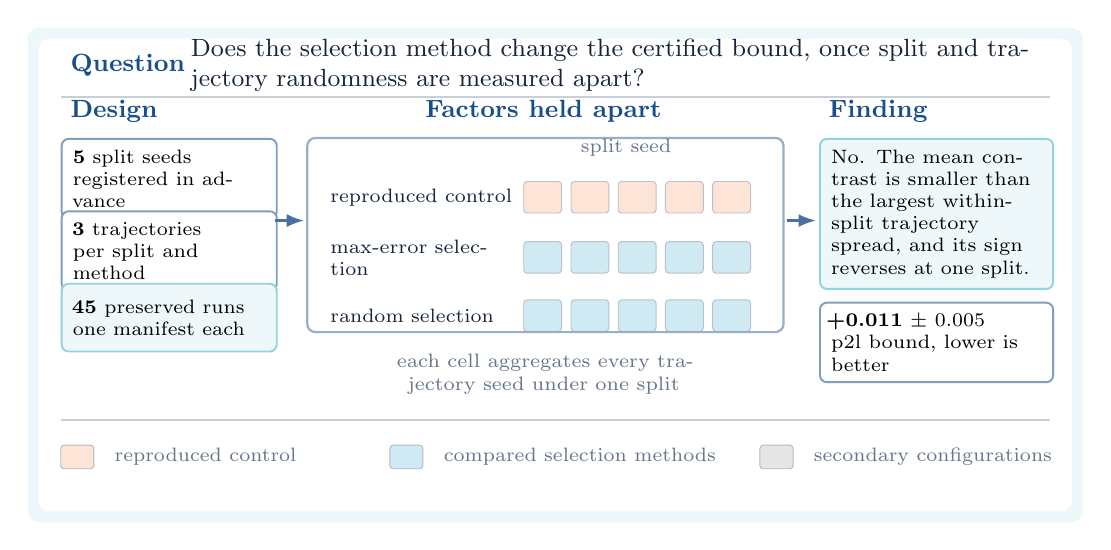
\begin{tikzpicture}[x=1cm,y=1cm,font=\sffamily]
    % ---- band 1: the question ------------------------------------------
    \node[anchor=west,font=\bfseries\small,text=ACBlue] at (0.42,5.12) {Question};
    \node[anchor=west,font=\small,text=ACInk,text width=10.8cm,align=left]
      at (1.95,5.12) {\TSquestion};
    \draw[ACMuted!35,line width=0.5pt] (0.42,4.72) -- (12.98,4.72);

    % ---- column titles ---------------------------------------------------
    \node[anchor=base west,font=\bfseries\small,text=ACBlue] at (0.42,4.46) {Design};
    \node[anchor=base,font=\bfseries\small,text=ACBlue] at (6.55,4.46)
      {Factors held apart};
    \node[anchor=base west,font=\bfseries\small,text=ACBlue] at (10.05,4.46) {Finding};

    % ---- left column: the registered design ------------------------------
    \node[acbox,anchor=north west,text width=2.45cm,minimum height=0.86cm,align=left,
          font=\scriptsize] (herodesign1) at (0.42,4.20)
      {\textbf{\TSsplitseeds} split seeds\\registered in advance};
    \node[acbox,anchor=north west,text width=2.45cm,minimum height=0.86cm,align=left,
          font=\scriptsize] (herodesign2) at (0.42,3.28)
      {\textbf{\TStrajper} trajectories\\per split and method};
    \node[acsoft,anchor=north west,text width=2.45cm,minimum height=0.86cm,align=left,
          font=\scriptsize] (herodesign3) at (0.42,2.36)
      {\textbf{\TSruns} preserved runs\\one manifest each};

    % ---- centre: the factor matrix ---------------------------------------
    % Structure only. Cells carry factor identity, not values, so nothing here
    % can be read as a magnitude that was never measured.
    %
    % \heroArms is a label/tint pair per row. Add a row here for a fourth or
    % fifth comparison arm; nothing else in this file needs to change. Each
    % row's vertical slot is measured from the label actually typeset in it
    % (`let` against the node's own north/south), not assumed to be one line:
    % a name too long for 2.35cm wraps to two lines and the row grows to fit
    % it, so a wrapped label can never clip into the row above, the row
    % below, or the matrix border.
    \def\heroArms{{\methodcontrol}/ACCompare,{\methodmax}/ACPrimary,{\methodrandom}/ACPrimary}
    \pgfmathsetlengthmacro{\heroMatrixTop}{4.20cm}
    \pgfmathsetlengthmacro{\heroCellH}{0.40cm}
    \pgfmathsetlengthmacro{\heroRowGap}{0.18cm}
    \pgfmathsetlengthmacro{\heroCursorY}{\heroMatrixTop-0.52cm}
    \foreach \heroLab/\heroTint [count=\heroI] in \heroArms {
      % text width is a cap: a name longer than fits on one line wraps here,
      % never past the label column and into the cell grid.
      \node[anchor=north west,font=\scriptsize,text=ACInk,text width=2.35cm,align=left]
        (herorowlab-\heroI) at (3.72,\heroCursorY) {\heroLab};
      \path let \p1=(herorowlab-\heroI.north), \p2=(herorowlab-\heroI.south)
        in \pgfextra{\xdef\heroLabTopRaw{\y1}\xdef\heroLabBotRaw{\y2}};
      \pgfmathsetlengthmacro{\heroLabH}{\heroLabTopRaw-\heroLabBotRaw}
      \pgfmathsetlengthmacro{\heroSlotH}{max(\heroLabH,\heroCellH)}
      \pgfmathsetlengthmacro{\heroCellTop}{\heroCursorY-(\heroSlotH-\heroCellH)/2}
      \pgfmathsetlengthmacro{\heroCellBot}{\heroCellTop-\heroCellH}
      \foreach \heroC in {0,1,2,3,4}{
        \fill[\heroTint,rounded corners=1.2pt]
          (6.30+\heroC*0.60,\heroCellBot) rectangle +(0.48,\heroCellH);
        \draw[ACMuted!45,line width=0.35pt,rounded corners=1.2pt]
          (6.30+\heroC*0.60,\heroCellBot) rectangle +(0.48,\heroCellH);
      }
      % \pgfmathsetlengthmacro defines \heroCursorY inside this iteration's
      % own group; re-exporting it with \global\let is what lets the next
      % iteration see the advanced value instead of the loop's start value.
      \pgfmathsetlengthmacro{\heroCursorY}{\heroCursorY-\heroSlotH-\heroRowGap}
      \global\let\heroCursorY\heroCursorY
    }
    \pgfmathsetlengthmacro{\heroLastRowBot}{\heroCursorY+\heroRowGap}
    \coordinate (heromatrixtl) at (3.55,\heroMatrixTop);
    \coordinate (heromatrixbr) at (9.60,\heroLastRowBot);
    \node[fit=(heromatrixtl)(heromatrixbr),draw=ACBlue!45,line width=0.8pt,
          rounded corners=3pt,inner sep=0pt] (heromatrixbox) {};
    % Every offset below is written with an explicit `cm` because it is
    % combined, via subtraction, with a `pgfmathsetlengthmacro` result: pgf
    % arithmetic between an explicit-unit length and a bare number treats
    % the bare number as bare points, not as a multiple of the picture's
    % x=1cm/y=1cm basis -- a dropped `cm` here silently shrinks a 0.36cm gap
    % to 0.36pt. (This is exactly the bug an earlier draft of this file hit:
    % the split-seed axis label collapsed onto the header above it.)
    \node[anchor=south,font=\scriptsize,text=ACMuted] at (7.60,\heroMatrixTop-0.36cm) {\splitseed};
    \node[anchor=north,font=\scriptsize,text=ACMuted,text width=6.4cm,align=center]
      (heromatrixcaption) at (6.55,\heroLastRowBot-0.16cm)
      {each cell aggregates every \trajseed\ under one split};
    \draw[acarrow] (3.14,3.15) -- (3.51,3.15);

    % ---- right column: the supported takeaway ----------------------------
    % No minimum height on the Finding box: it sizes to \TSfinding, however
    % long the supported sentence is. The delta box is anchored below it
    % (`positioning`'s below=of), so the two can never overlap regardless of
    % how tall the finding grows.
    \node[acsoft,anchor=north west,text width=2.68cm,minimum height=0.86cm,align=left,
          font=\scriptsize] (herofinding) at (10.05,4.20) {\TSfinding};
    \node[acbox,text width=2.68cm,minimum height=0.85cm,align=left,font=\scriptsize,
          below=0.15cm of herofinding] (herodelta)
      {\textbf{\TSdelta} $\pm$ \TSdeltaunc\\\TSmetric, lower is better};
    \draw[acarrow] (9.64,3.15) -- (10.01,3.15);

    % ---- everything below the three columns is measured, not assumed -----
    % The lowest of {left design column, matrix + its caption, finding +
    % delta} sets where the legend band starts. Whichever column is tallest
    % this time is the one that governs; the other two just have slack.
    \node[fit=(herodesign3)(heromatrixcaption)(herodelta),inner sep=0pt]
      (herocontentbottom) {};
    \path let \p1 = (herocontentbottom.south)
      in \pgfextra{\xdef\heroContentBottomRaw{\y1}};
    \pgfmathsetlengthmacro{\heroLegendLineY}{\heroContentBottomRaw-0.20cm}
    \pgfmathsetlengthmacro{\heroSwatchTopY}{\heroLegendLineY-0.32cm}
    \pgfmathsetlengthmacro{\heroSwatchBotY}{\heroSwatchTopY-0.30cm}
    \pgfmathsetlengthmacro{\heroFrameBotY}{\heroSwatchBotY-0.68cm}
    \pgfmathsetlengthmacro{\heroFrameInnerBotY}{\heroFrameBotY+0.14cm}

    % ---- band 3: the visual key later figures reuse ----------------------
    \draw[ACMuted!35,line width=0.5pt] (0.42,\heroLegendLineY) -- (12.98,\heroLegendLineY);
    \foreach \x/\tint/\lab in {%
      0.42/ACCompare/{\methodcontrol},
      4.60/ACPrimary/{compared selection methods},
      9.30/ACNeutral/{secondary configurations}}{
      \fill[\tint,rounded corners=1.2pt] (\x,\heroSwatchBotY) rectangle +(0.42,0.30);
      \draw[ACMuted!50,line width=0.35pt,rounded corners=1.2pt]
        (\x,\heroSwatchBotY) rectangle +(0.42,0.30);
      \node[anchor=west,font=\scriptsize,text=ACMuted] at (\x+0.56,\heroSwatchTopY-0.15cm) {\lab};
    }

    % ---- frame ------------------------------------------------------------
    % Drawn last but placed behind everything (background layer), sized to
    % whatever the content above actually needed. In the common case (three
    % rows, a one-line finding) this reproduces the original fixed 0..5.6
    % card exactly; it only grows when a row or a finding needs the room.
    \begin{scope}[on background layer]
      \fill[ACPrimary!35,rounded corners=4pt] (0,\heroFrameBotY) rectangle (13.4,5.6);
      \fill[white,rounded corners=4pt] (0.14,\heroFrameInnerBotY) rectangle (13.26,5.46);
    \end{scope}
  \end{tikzpicture}%
  }
\end{center}

\vspace{-3mm}

\begin{abstract}
% Abstract. One paragraph, 140-190 words, no citations, no display math.
% Drafted last. Every number here also appears in tables/main_results.tex.
Disagreement-based generalization bounds certify a target model through a
simpler \surrogate, paying for the substitution with a term that measures how
often the two disagree on unlabeled data. Which examples the \surrogate\ is
built from is left open by the theory, and published comparisons between
selection strategies mix the effect of the method with the effect of the data
split and the optimization path that produced each run. We freeze the \evalsem\
that give the bound its meaning, register a comparison matrix before running it,
and vary the \splitseed\ and the \trajseed\ independently across \methodrandom\
and \methodmax. Over 5 \splitseed{}s and 3 trajectory seeds per split and
method, \methodrandom\ attains a lower mean \certbound\ by $0.011 \pm 0.005$.
That contrast is smaller than the largest within-split trajectory spread of
$0.032$, and its sign reverses at one split, so the two strategies are
indistinguishable at this scale. On this dataset and at this scale, the
optimization path dominates the selection criterion.

\end{abstract}

% Introduction. Contract: ../references/section-playbook.md
% 420-650 words, four paragraphs, then 2-4 contribution items.
\section{Introduction}
\label{sec:introduction}

% P1 - problem
Certifying how a trained network will behave on unseen data is the point at
which a great deal of applied machine learning stops being measurable. Bounds
that are tight enough to be informative on realistic architectures have been
difficult to obtain directly~\cite{livni2020limitation, hellstrm2023generalization},
and the constructions that do succeed tend to route around the target model
rather than through it. Compression-based arguments certify a network by
certifying a smaller description of it~\cite{arora2018stronger, zhou2018nonvacuous,
shin2021compressing, bazinet2024sample}. Disagreement-based arguments go one
step further: they bound a tractable \surrogate, then bound how often the
\surrogate\ and the target disagree on unlabeled data, and combine the two into
a certificate for the target~\cite{jiang2021assessing, kirsch2022assessing}.
The appeal is that both halves are measurable even when the target is not.

% P2 - gap
The construction leaves one choice to the practitioner: which examples the
\surrogate\ is built from. Selection strategies for this role are well studied
in their own right, from uniform sampling through error-aware and
disagreement-aware criteria~\cite{coleman2019selection, xia2023refined,
benkert2024effective, feng2024tarot}, and they differ in how much control they
exert over the quantity the bound depends on. It would be natural to expect the
strategy with the most direct control over disagreement to produce the tightest
certificate. Reported comparisons do not consistently show that. However, the
evidence behind those comparisons mixes at least three sources of variation:
which data split was drawn, which selection method was used, and which
optimization path the training run happened to take. A single number cannot
separate them, so the observation is currently a result about a set of runs
rather than a result about a method.

% P3 - what this paper does
This paper measures the three factors apart. We freeze the \evalsem\ that give
the bound its meaning, register a comparison matrix before running it, and vary
the \splitseed\ and the \trajseed\ independently across the compared selection
methods. Contrasts are taken within a split, so the split effect cancels by
construction rather than by assumption, and a reporting threshold fixed before
execution decides whether a contrast is large enough to be called a finding at
all. Every run is preserved with a manifest identifying its method, seeds,
configuration, and exact command, so each reported statistic traces back to the
primary runs it aggregates.

% P4 - result and scope
Across 5 \splitseed{}s and 3 trajectory seeds per split and method, \methodrandom\
attains a lower mean \certbound\ than \methodmax\ by $0.011 \pm 0.005$. That
contrast does not clear the largest within-split trajectory spread in the
matrix, $0.032$, and its sign reverses at one of the five splits. The supported
conclusion is therefore that the two strategies are indistinguishable at this
scale, and that the trajectory, not the selection method, is the dominant
source of variation in the certificate. This is measured on one dataset at a
reduced experimental scale; it is not a claim about selection strategies in
general.

Our contributions are as follows:
\begin{itemize}[itemsep=0.5ex, parsep=0pt, topsep=0pt]
\item[\textbf{(1)}] A factorial design that separates \splitseed, selection
method, and \trajseed\ under frozen \evalsem, together with a reporting
threshold fixed in advance, which makes a method-level comparison identifiable
rather than confounded.

\item[\textbf{(2)}] A measurement of how large the trajectory-induced spread in
a disagreement-based certificate actually is, and the finding that it exceeds
the between-method contrast at this scale.

\item[\textbf{(3)}] A provenance-preserving pipeline in which every reported
aggregate enumerates the primary runs it was computed from, so any number in
the paper can be checked against a preserved record.
\end{itemize}

% Related Work. Contract: ../references/section-playbook.md
% 420-650 words, thematic paragraphs, each ending by positioning this work.
\section{Related Work}
\label{sec:related-work}

\textbf{Certificates that route around the target model.}
PAC-Bayesian analysis supplies most of the machinery behind non-vacuous bounds
for over-parameterised networks, and a long line of work has sharpened
it: fast-rate forms~\cite{yang2019fastrate, grnwald2021pacbayes}, extensions to
unbounded losses~\cite{casado2024pacbayeschernoff}, non-i.i.d.\ data~\cite{ralaivola2009chromatic},
meta-learning~\cite{farid2021generalization, leblanc2024generalization}, and
data-dependent priors~\cite{dziugaite2018datadependent, pitas2022posteriors}.
Broader surveys connect these guarantees to information-theoretic
quantities~\cite{hellstrm2023generalization}, and negative results delimit what
the framework can deliver at all~\cite{livni2020limitation}. A second family
certifies the target by certifying a compressed description of
it~\cite{arora2018stronger, zhou2018nonvacuous, shin2021compressing,
guha2023generalization, bazinet2024sample}, sometimes using coresets as the
compression mechanism~\cite{baykal2018datadependent}. Both families share a
structural feature that matters here: the certificate is assembled from a
\surrogate\ object, and the quality of that object is a modelling choice rather
than a consequence of the theory.

\textbf{Disagreement as the bridging term.}
Disagreement between independently trained models is a surprisingly accurate
predictor of generalization~\cite{jiang2021assessing}, though the explanation
for why is contested~\cite{kirsch2022assessing}. The quantity has since been
used as a training signal in domain generalization~\cite{zhang2022adaptive},
as a selection criterion for annotation~\cite{benkert2024effective}, and as a
supervision signal in its own right~\cite{daniels2025diverse}. Used inside a
certificate, disagreement plays a different role: it is the term that transfers
a guarantee from the \surrogate\ to the target, and it is measured on unlabeled
data rather than optimized against a held-out label set. That distinction is
what makes the selection question sharp, because the same choice that lowers
the disagreement estimate also changes the \surrogate\ whose guarantee is being
transferred.

\textbf{Which examples the \surrogate\ is built from.}
Coreset construction offers a large menu of principled
answers~\cite{jubran2019introduction, blmer2016coreset, maalouf2021unified,
jaiswal2023universal, chhaya2020coresets, jourdan2025coreset, chen2024tuningfree},
and the deep learning literature adds selection criteria driven by proxy
models~\cite{coleman2019selection}, performance constraints~\cite{xia2023refined},
optimal transport~\cite{feng2024tarot}, pruning~\cite{kousar2025pruningbased},
and information-theoretic arguments~\cite{foggo2019analyzing}; recent surveys
cover the space at scale~\cite{albalak2024survey}. These strategies are
routinely compared by the downstream metric they produce. The comparisons are
usually reported at a single data split and a single training run, which leaves
the method effect entangled with the randomness of the run that produced it.

\textbf{How much of a reported difference is the seed.}
Seed-to-seed variation is large enough to change conclusions in fine-tuning
regimes~\cite{bui2025assessing}, in certified robustness~\cite{le2026extreme},
and in training-variance studies more
generally~\cite{steier2026margin, sun2026varianceaware}; variance-aware training
procedures exist partly because of it~\cite{zantedeschi2021stochastic,
viallard2024leveraging, warrell2022higherorder}. What is missing is the same
measurement for a disagreement-based certificate, where two distinct sources of
randomness act on the reported number through different paths.

\textbf{Scope of this paper.}
Prior work reports method-level outcomes for selection strategies, and separately
establishes that seed variance is large. This paper measures the two together on
one certificate, under one frozen evaluation, and reports the full matrix rather
than its most favorable cell.

% Method. Contract: ../references/section-playbook.md and equation-grammar.md
% 1300-2100 words, 3-4 subsections, at least 4 numbered equations.
% The overview figure is the first thing in the section, before any equation.
\section{Method}
\label{sec:method}
% Tier C structural overview. First float of the Method section, placed before
% the section's first equation. Carries no magnitudes: it states what is fixed,
% what varies, and what the paper reports.
\begin{figure*}[t]
  \centering
  \resizebox{0.99\textwidth}{!}{%
  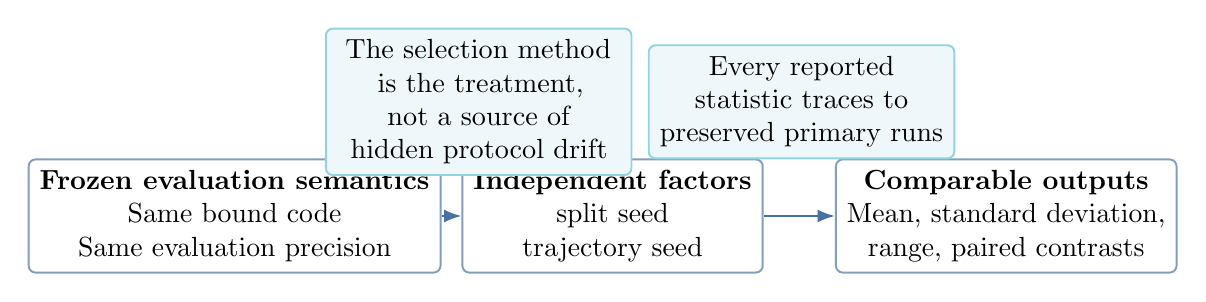
\begin{tikzpicture}[x=1cm,y=1cm]
    \node[acbox,minimum width=3.5cm,minimum height=1.15cm,align=center] (a) at (1.9,1.1)
      {\textbf{Frozen \evalsem}\\Same bound code\\Same evaluation precision};
    \node[acbox,minimum width=3.5cm,minimum height=1.15cm,align=center] (b) at (6.7,1.1)
      {\textbf{Independent factors}\\\splitseed\\\trajseed};
    \node[acbox,minimum width=3.7cm,minimum height=1.15cm,align=center] (c) at (11.7,1.1)
      {\textbf{Comparable outputs}\\Mean, standard deviation,\\range, paired contrasts};
    \draw[acarrow] (a) -- (b);
    \draw[acarrow] (b) -- (c);
    % text width is a cap, not a floor: at this 4.1cm center spacing the two
    % callouts can grow only downward (more lines), never sideways into each
    % other, regardless of how long the caption text is.
    \node[acsoft,text width=3.6cm,align=center] at (5.0,2.55)
      {The selection method is the treatment, not a source of hidden protocol
       drift};
    \node[acsoft,text width=3.6cm,align=center] at (9.1,2.55)
      {Every reported statistic traces to preserved primary runs};
  \end{tikzpicture}}
  \caption{\textbf{Study design.} The evaluation is fixed before any comparison
    begins, the two sources of randomness are varied independently, and the
    reported statistics are defined in advance. Fixing the left panel is what
    makes the right panel a measurement of the method rather than of the
    protocol.}
  \label{fig:overview}
\end{figure*}


\subsection{Setting and notation}
\label{sec:setting}

A disagreement-based certificate bounds the risk of a target model through a
simpler \surrogate\ that admits a computable guarantee.
\Cref{fig:overview} summarizes the design: the evaluation is fixed first, the
two sources of randomness are varied independently, and the reported statistics
are defined before any comparison is run. We write one evaluation instance as a
tuple $(\mathcal{S}, m, \tau) \rightarrow \bnd$, where $\mathcal{S}$ is the data
split, $m$ the selection method that determines which examples the \surrogate\
is built from, $\tau$ the \trajseed\ that fixes the optimization path, and
$\bnd$ the resulting \certbound. Lower $\bnd$ is better.

The certificate has two parts that move in opposite directions when the
selection method changes, which is the reason a selection effect is not
self-evident:
\begin{equation}\label{eq:certificate}
  \bnd \;=\; \underbrace{\mathcal{C}(\hypclass)}_{\text{\surrogate\ guarantee}}
  \;+\;
  \underbrace{\widehat{d}(\dataset_u)}_{\text{\disagreement}},
\end{equation}
where $\mathcal{C}(\hypclass)$ is the \surrogate's own guarantee, which depends
on its complexity relative to its prior, and $\widehat{d}(\dataset_u)$ is the
estimated disagreement between target and \surrogate\ measured on an unlabeled
set $\dataset_u$. \Cref{eq:certificate} is what makes the comparison in this
paper non-trivial: a selection method that reduces the second term by fitting
$\dataset_u$ more aggressively can enlarge the first by more than it gains, and
the observed $\bnd$ reports only the sum. Neither term is separately reported by
the pipeline, so a method comparison at the level of $\bnd$ cannot attribute a
difference to one term or the other without additional instrumentation.

Three things are fixed for every run reported in this paper: the bound
computation itself, the evaluation precision, and the split boundaries between
training, validation, disagreement, and test data. Changing any of them makes
numbers on either side of the change incomparable, so they are frozen before the
matrix is registered and are never treated as tunable. Concretely, the
confidence parameter is $\delta = 0.05$, the bound-inversion grid holds 1000
points, the Monte Carlo estimate of the \disagreement uses 10{,}000 samples,
and the four-way split is drawn once per \splitseed\ and reused by every method
at that split. The training and disagreement partitions never overlap.

\subsection{The compared selection methods}
\label{sec:methods}

The two selection methods differ in exactly one respect: the criterion used to
choose the examples the \surrogate\ is fitted on. \methodrandom\ draws them
uniformly without replacement from the training partition. \methodmax\ ranks
candidates by the target model's loss and takes the highest-loss examples, which
is the strategy with the most direct control over the region where target and
\surrogate\ are most likely to disagree. Both draw the same number of examples,
run for the same number of epochs, use the same optimizer and schedule, and are
evaluated by the same frozen code path. The \methodcontrol\ is the unmodified
upstream pipeline, re-run and recorded in this environment rather than quoted
from a prior publication, because published numbers came from different
hardware, a different epoch budget, and full-precision evaluation.

Holding the budget equal needs saying precisely, because the two criteria
consume it differently. Both arms select the same number of examples and train
for the same number of epochs on them, so the \surrogate\ sees the same number
of gradient steps in both. \methodmax\ additionally requires a forward pass over
the training partition to rank candidates by target loss, which is a one-time
cost outside the training loop and is not charged against the epoch budget. That
asymmetry favours \methodmax\ in wall-clock terms and is irrelevant to the
certificate, which depends on the fitted \surrogate\ and not on how its training
set was chosen. We report it because a budget claim that is only true of one
resource is the kind of detail that makes two studies incomparable later.

This is a deliberately narrow contrast. Richer strategies exist, including
disagreement-aware and hybrid criteria, and they are not evaluated here. The
narrow contrast is what makes the identification argument in the next subsection
possible: two arms that differ in one criterion, run over the same splits with
the same budget, admit an exact pairing that a broader sweep would not.

\subsection{Separating the factors}
\label{sec:factors}

A comparison between two selection methods is identifiable only if the remaining
sources of variation are either held fixed or averaged over. We therefore treat
each observed bound as the sum of a split effect and a trajectory residual under
that split:
\begin{equation}\label{eq:decomposition}
  \bnd_{\splitidx\trajidx}^{(m)}
  \;=\;
  \mu^{(m)} + \alpha_{\splitidx} + \varepsilon_{\splitidx\trajidx}^{(m)},
  \qquad
  \textstyle\sum_{\splitidx} \alpha_{\splitidx} = 0,
\end{equation}
where $\bnd_{\splitidx\trajidx}^{(m)}$ is the bound obtained by method $m$ at
\splitseed\ $\splitidx$ and \trajseed\ $\trajidx$, $\mu^{(m)}$ is the method's
grand mean, $\alpha_{\splitidx}$ is the effect of the split itself, shared by all
methods, and $\varepsilon_{\splitidx\trajidx}^{(m)}$ is the trajectory residual.
\Cref{eq:decomposition} states the identification problem directly: a difference
between methods measured at different splits confounds $\mu^{(m)}$ with
$\alpha_{\splitidx}$, so it is not evidence about the method.

\textbf{Design rule}: \textit{a method contrast is reported only when it is
measured within a split, and a method ranking is reported only when it is
consistent across splits.}

Both halves of that rule matter. The first removes $\alpha_{\splitidx}$ from the
contrast by construction rather than by assumption. The second prevents a
ranking that holds at one split and reverses at another from being reported as a
property of the method, which is the failure mode that a single-split comparison
cannot detect. The rule is restrictive on purpose: it can leave a study with a
measured contrast and no ranking to report, and that outcome is a result rather
than a shortfall.

\subsection{Estimators and uncertainty}
\label{sec:estimators}

For each method $m$ and \splitseed\ $\splitidx$ we run $T$ trajectory seeds and
summarize them by their mean and their spread:
\begin{equation}\label{eq:persplit}
  \bar{\bnd}^{(m)}_{\splitidx} = \frac{1}{T}\sum_{\trajidx=1}^{T}
    \bnd^{(m)}_{\splitidx\trajidx},
  \qquad
  s^{(m)}_{\splitidx} = \sqrt{\frac{1}{T-1}\sum_{\trajidx=1}^{T}
    \bigl(\bnd^{(m)}_{\splitidx\trajidx} - \bar{\bnd}^{(m)}_{\splitidx}\bigr)^2},
\end{equation}
where $T$ is the number of trajectory seeds per split,
$\bar{\bnd}^{(m)}_{\splitidx}$ the per-split mean, and $s^{(m)}_{\splitidx}$ the
trajectory standard deviation under a fixed split. \Cref{eq:persplit} is the
unit of evidence in this paper: a single trajectory is an observation, and only
$\bar{\bnd}^{(m)}_{\splitidx}$ with its spread is quoted as a result. The spread
is reported alongside the mean everywhere the mean appears, including in the
abstract, because the two numbers answer different questions and the first is
uninterpretable without the second.

The headline comparison is the paired contrast between two methods, taken within
split and trajectory index so that both $\alpha_{\splitidx}$ and any shared
trajectory effect cancel:
\begin{equation}\label{eq:contrast}
  \Delta_{\splitidx} = \bar{\bnd}^{(m_1)}_{\splitidx} - \bar{\bnd}^{(m_2)}_{\splitidx},
  \qquad
  \bar{\Delta} = \frac{1}{S}\sum_{\splitidx=1}^{S} \Delta_{\splitidx},
\end{equation}
where $S$ is the number of \splitseed{}s, $\Delta_{\splitidx}$ the within-split
contrast, and $\bar{\Delta}$ its mean across splits. \Cref{eq:contrast} is the
quantity reported in the main results table; the per-split $\Delta_{\splitidx}$
are reported alongside it so that a mean contrast cannot hide a reversal.

Finally, a contrast is only reported as a finding when it exceeds the noise it is
measured against:
\begin{equation}\label{eq:decision}
  \bigl|\bar{\Delta}\bigr| \;>\; \kappa \cdot
  \max_{m,\splitidx}\, s^{(m)}_{\splitidx},
  \qquad \kappa = 1.0,
\end{equation}
where $\kappa$ is a threshold fixed before the matrix was run and
$\max_{m,\splitidx} s^{(m)}_{\splitidx}$ is the largest within-split trajectory
spread observed anywhere in the matrix. The threshold is expressed against an observed spread rather than against a
distributional assumption because the quantity in question, the movement of a
certificate under a change of \trajseed, has no established parametric form here
and only three observations per cell from which to estimate one.
\Cref{eq:decision} is a stopping rule rather than a significance test: when it fails, the finding this paper reports is
that the methods are indistinguishable at this scale, and that statement is
recorded rather than replaced by a smaller comparison that happens to pass. The
comparison against the largest observed spread, rather than against the spread of
the winning arm, is the conservative choice; \cref{sec:appendix-statistics}
reports what the verdict would have been under the alternatives.

\subsection{Provenance}
\label{sec:provenance}

Every run writes a raw result together with a manifest recording its method,
source script and revision, exact command, dataset, \splitseed, \trajseed, full
configuration, timestamps, and environment. Aggregates enumerate the primary run
paths they were computed from. A quantity whose primary record is missing,
overwritten, or method-ambiguous is excluded from the main paper rather than
reported with a caveat. This matters in practice because the upstream pipeline
names its output files from hyperparameters alone, so two different methods run
at the same hyperparameters write to the same filename and the second silently
overwrites the first. The aggregation step reads only manifests and raw results. It refuses to write
an aggregate when a listed primary input is absent from disk, so a broken
evidence chain surfaces as a failure at aggregation time rather than as a
plausible number in a table. Each aggregate stores the estimator it applied, the
per-seed values it combined, and the paths it combined them from, which is what
makes a reported statistic checkable rather than merely reproducible in
principle. \Cref{sec:appendix-provenance} gives the manifest schema and the
aggregation procedure in full.

% Experiments. Contract: ../references/section-playbook.md
% 600-1000 words in four subsections: setup, main results, distribution, ablations.
\section{Experiments}
\label{sec:experiments}

\subsection{Experimental setup}
\label{sec:setup}

\textbf{Data and evaluation.}
All runs use MNIST with the upstream four-way partition into training,
validation, disagreement, and test sets. The \evalsem\ are frozen as described in
\cref{sec:setting}: $\delta = 0.05$, a 1000-point bound-inversion grid, and
10{,}000 Monte Carlo samples for the disagreement estimate. These values are
identical for every run below and were fixed before the comparison matrix was
registered.

\textbf{Scale.}
Runs use a reduced probe scale of 12 epochs and a maximum compression size of
120, against the upstream configuration's 200 epochs and 20{,}000. Scale is a
free parameter of this study, but it is applied identically on both sides of
every comparison, so a change in scale cannot produce a difference between
methods. \Cref{tab:scale} reports what changes when the compression budget is
doubled.

\textbf{Compared configurations.}
\tightcolorbox{ACCompare}{\textbf{\methodcontrol.}} The unmodified pipeline,
re-run and recorded in this environment.
\tightcolorbox{ACPrimary}{\textbf{Selection methods.}} \methodmax\ and
\methodrandom, differing only in which examples the \surrogate\ is built from,
as described in \cref{sec:methods}.

\textbf{Seeds and repetition.}
5 \splitseed{}s $\{1,2,3,4,42\}$, 3 trajectory seeds per split and method, giving
45 preserved primary runs. Statistics follow \cref{eq:persplit} and
\cref{eq:contrast}; the reporting threshold of \cref{eq:decision} was fixed at
$\kappa = 1.0$ before execution.

\textbf{Environment and failure handling.}
All runs executed on a single GPU under one dependency lock, recorded in each run
manifest and reproduced in \cref{sec:appendix-config}. No run in the reported
matrix crashed. Crashed runs, had there been any, would be preserved with their
manifests and counted rather than silently retried or dropped from the
denominator.

\subsection{Main results}
\label{sec:main-results}

% Mandatory main results table. Contract: references/table-grammar.md, pattern 1.
% Every cell is filled from runs/aggregate__<method>.json.
\begin{table}[t!]
  \caption{\textbf{\certbound\ (\down) under the frozen protocol.}
    \swatch{ACCompare} is the \methodcontrol,
    \swatch{ACPrimary} are the compared selection methods.
    Mean is over 5 \splitseed{}s, each aggregating 3 trajectory seeds under
    identical \evalsem. Std.\ is the standard deviation of the per-split means
    and Range is their max\,$-$\,min; both describe variation \emph{between}
    splits, not within one. The paired contrast is computed against the
    \methodcontrol\ within split and trajectory index, following
    \cref{eq:contrast}; ``--'' marks the row a contrast is taken against.}
  \label{tab:main-results}
  \vspace{-0.2cm}
  \centering
  {\fontsize{8pt}{11pt}\selectfont
   \resizebox{\linewidth}{!}{%
     \begin{NiceTabular}{l c c c c c c c}[colortbl-like]
       \toprule[1.2pt]
         & \begin{tabular}{c}\textbf{Split}\\\textbf{seeds}\end{tabular}
         & \begin{tabular}{c}\textbf{Traj.}\\\textbf{per split}\end{tabular}
         & \textbf{Mean}
         & \textbf{Std.}
         & \textbf{Range}
         & \begin{tabular}{c}\textbf{Max traj.}\\\textbf{std.}\end{tabular}
         & \begin{tabular}{c}\textbf{Paired}\\\textbf{contrast}\end{tabular} \\
       \midrule[1.2pt]\midrule
       \rowcolor{ACCompare}\methodcontrol
         & 5 & 3 & 0.409 & 0.007 & 0.019 & 0.019 & -- \\
       \midrule
       \rowcolor{ACPrimary}\methodmax
         & 5 & 3 & 0.398 & 0.009 & 0.024 & 0.023 & $-0.011$ \\
       \rowcolor{ACPrimary}\methodrandom
         & 5 & 3 & 0.387 & 0.013 & 0.030 & 0.032 & $-0.022$ \\
       \bottomrule
     \end{NiceTabular}
   }
  }
\end{table}


\textbf{Does the selection method change the \certbound?}
\Cref{tab:main-results} gives the aggregate view. Both selection methods improve
on the \methodcontrol: \methodmax\ by $0.011$ and \methodrandom\ by $0.022$ in
paired within-split contrast. Between the two selection methods the paired
contrast is $0.011 \pm 0.005$ in favour of \methodrandom. The largest within-split
trajectory spread anywhere in the matrix is $0.032$, so by \cref{eq:decision} the
between-method contrast does not clear the noise it is measured against. The
supported statement is that the two methods are indistinguishable at this scale,
with a direction that favours \methodrandom\ but is not established.

\textbf{Is the ordering stable across splits?}
% Mandatory secondary table. Contract: references/table-grammar.md, pattern 2.
\begin{table}[t!]
  \caption{\textbf{Per-split \certbound\ and paired contrast (\down).} Each
    column is one \splitseed. Every entry is the mean over the same three
    trajectory seeds, so the difference row is an exact pairing. A positive
    difference favors \methodrandom. The sign reverses at \splitseed~42, which
    is why \cref{tab:main-results} reports a contrast and not a ranking.}
  \label{tab:paired}
  \vspace{-0.2cm}
  \centering
  {\fontsize{8pt}{11pt}\selectfont
     \begin{NiceTabular}{l c c c c c}[colortbl-like]
       \toprule[1pt]
       \textbf{\splitseed} & \textbf{1} & \textbf{2} & \textbf{3} & \textbf{4} & \textbf{42} \\
       \midrule
       \methodcontrol & 0.412 & 0.405 & 0.418 & 0.399 & 0.410 \\
       \methodmax     & 0.401 & 0.395 & 0.412 & 0.388 & 0.394 \\
       \rowcolor{ACPrimary}\methodrandom & 0.379 & 0.384 & 0.398 & 0.371 & 0.401 \\
       \midrule
       Difference     & 0.022 & 0.011 & 0.014 & 0.017 & $-0.007$ \\
       \bottomrule
     \end{NiceTabular}
  }
\end{table}

\Cref{tab:paired} reports the same comparison split by split. The contrast
favours \methodrandom\ at four of the five splits and reverses at \splitseed~42,
where \methodmax\ is lower by $0.007$. Under the design rule of
\cref{sec:factors}, a ranking requires consistency across splits, so no ranking
is reported. A mean contrast computed over splits whose individual contrasts
disagree in sign describes the sample, not the method.

Notice also that the between-split range grows monotonically with how aggressively
the method selects: $0.019$ for the \methodcontrol, $0.024$ for \methodmax, and
$0.030$ for \methodrandom. Whatever a selection criterion does to the mean, it
also changes how much the certificate moves when the split changes, and the
latter effect is the larger one here.

\subsection{Trajectory variation}
\label{sec:trajectory}

\IfFileExists{data/bounds.dat}{%
  % Tier B results figure: pgfplots reading a data file written by the analysis
% script. Guarded with \IfFileExists so that, before the data exists, the float
% does not appear at all (Tier D of references/figure-ladder.md).
%
% source-data: runs/aggregate__{control,maxerr,random}.json -> paper/data/bounds.dat
% generator:   scripts/make_paper_data.py --figure distribution
\begin{figure}[!t]
  \centering
  \begin{tikzpicture}
    \begin{axis}[acplot,
      xlabel={\splitseed}, ylabel={\certbound\ $\downarrow$},
      xtick=data, symbolic x coords={1,2,3,4,42},
      enlarge x limits=0.12,
    ]
      \addplot[name path=lo,draw=none,forget plot] table[x=seed,y=rlo] {data/bounds.dat};
      \addplot[name path=hi,draw=none,forget plot] table[x=seed,y=rhi] {data/bounds.dat};
      \addplot[ACBlue!14,forget plot] fill between[of=lo and hi];
      \addplot+[ACMuted, mark=triangle*, dashed]
        table[x=seed,y=control] {data/bounds.dat};
      \addplot+[ACCompare!55!black, mark=square*]
        table[x=seed,y=maxerr] {data/bounds.dat};
      \addplot+[ACBlue, mark=*]
        table[x=seed,y=random] {data/bounds.dat};
      \legend{\methodcontrol, \methodmax, \methodrandom}
    \end{axis}
  \end{tikzpicture}
  \caption{\textbf{Per-split \certbound\ and trajectory spread.} Each marker is
    the mean over 3 trajectory seeds at a fixed \splitseed, under identical
    \evalsem; the shaded band is the trajectory range of \methodrandom. The band
    contains the \methodmax\ mean at every split, so the ordering visible in the
    means is not separable from trajectory noise. The comparison is read across
    splits, not at a single split: the ordering reverses at \splitseed~42.}
  \label{fig:distribution}
\end{figure}
%
  \Cref{fig:distribution} shows the per-split means for all three
  configurations, with the trajectory range of \methodrandom\ as a shaded band.
  The band is wide enough at every split to contain the corresponding
  \methodmax\ mean, which is the same conclusion \cref{eq:decision} reaches
  arithmetically.%
}{}

Within-split trajectory standard deviations range from $0.011$ to $0.032$ across
the matrix, and are systematically larger for \methodrandom\ than for the
\methodcontrol. Against that, the between-method contrast of $0.011$ is small. A
comparison at this scale that used a single trajectory per configuration would
have had roughly a one-in-three chance of reporting the opposite ordering, which
is the practical reason the matrix is specified with repetition rather than
breadth. Where an individual trajectory is discussed, it is discussed as an
example: a single optimization path is an observation about that run, not an
ablation result and not evidence about a policy.

\subsection{Ablations}
\label{sec:ablations}

% Paired ablation tables. Contract: references/table-grammar.md, pattern 3.
\begin{table}[t!]
  \centering
  \begin{minipage}{0.48\textwidth}
    \centering
    \captionsetup{justification=centering,singlelinecheck=false}
    \caption{\textbf{Effect of trajectory count (\down).}}
    \vspace{-0.1cm}
    \label{tab:trajectory-count}
    {\fontsize{8pt}{11pt}\selectfont
     \begin{NiceTabular}{l ccc}[colortbl-like]
       \toprule[1.2pt]
       \textbf{Statistic} & \textbf{1} & \textbf{2} & \textbf{3} \\
       \midrule[1.2pt]
       Mean \certbound       & 0.362 & 0.376 & 0.387 \\
       Between-split std.    & 0.013 & 0.013 & 0.013 \\
       Mean paired contrast  & 0.014 & 0.012 & 0.011 \\
       \bottomrule[1.2pt]
     \end{NiceTabular}%
    }
  \end{minipage}
  \hfill
  \begin{minipage}{0.44\textwidth}
    \centering
    \captionsetup{justification=centering,singlelinecheck=false}
    \caption{\textbf{Effect of experiment scale (\down).}}
    \vspace{-0.1cm}
    \label{tab:scale}
    {\fontsize{8pt}{11pt}\selectfont
     \begin{NiceTabular}{l ccc}[colortbl-like]
       \toprule[1.2pt]
       \textbf{Setting} & \textbf{Epochs} & \textbf{Comp.} & \textbf{Bound} \\
       \midrule[1.2pt]
       Reduced      &  12 &   120 & 0.387 \\
       Intermediate &  12 &   240 & 0.381 \\
       Original     & 200 & 20000 & --    \\
       \bottomrule[1.2pt]
     \end{NiceTabular}%
    }
  \end{minipage}
\end{table}


\Cref{tab:trajectory-count} varies the number of trajectory seeds aggregated per
split. The estimated mean drifts upward as trajectories are added, from $0.362$
at one trajectory to $0.387$ at three, while the between-split standard deviation
is unchanged at $0.013$ and the mean paired contrast shrinks from $0.014$ to
$0.011$. A one-trajectory estimate is therefore both optimistic about the bound
and generous about the contrast, in the direction that would most easily produce
a positive-sounding result. Three trajectories is where the contrast stops
moving, not where it clears the threshold of \cref{eq:decision}.

\Cref{tab:scale} compares compression budgets. Doubling the budget from 120 to
240 lowers the bound for \methodrandom\ by $0.006$, an effect of the same order
as the between-method contrast. The comparison at the upstream scale of 200
epochs and 20{,}000 was not run, and no value is reported for it.

% Conclusion. 180-320 words. Only gate-passed claims. No new numbers.
\section{Conclusion}
\label{sec:conclusion}

A comparison between selection strategies for a disagreement-based certificate
is identifiable only when the \splitseed\ and the \trajseed\ are varied
independently under frozen \evalsem. We registered that matrix before running
it, preserved every run with a manifest identifying its method and seeds, and
reported the full set of per-split contrasts rather than the most favorable one.

On MNIST at a reduced probe scale, \methodrandom\ and \methodmax\ are
indistinguishable. The mean paired contrast favours \methodrandom, but it is
smaller than the largest within-split trajectory spread in the matrix, and it
changes sign at one of the five splits. What the matrix does establish is the
size of the nuisance: the trajectory alone moves the certificate by more than
the selection criterion does, and the between-split range grows with how
aggressively a method selects. A study that reports one trajectory per
configuration is measuring that nuisance and attributing it to the method.

The scope is narrow by construction. One dataset, one certificate family, two
selection criteria, and a reduced experimental scale. The comparison at the
upstream scale of 200 epochs and 20{,}000 compression size was not run, and the
scale ablation shows an effect there of the same order as the between-method
contrast, so that comparison is the one most likely to change the answer.
Disagreement-aware and hybrid selection criteria are untested here and need the
same paired design rather than a single additional run. Whether the trajectory
spread narrows at full scale, or is an intrinsic property of the certificate, is
the question this design is now sized to answer.

\section*{Acknowledgments}
This document is a demonstration instance produced by the AutoConference
paper-writing skill. Its numbers are synthetic and describe no real experiment.


\clearpage
\bibliographystyle{plainnat}
\bibliography{references}

\clearpage
% Appendix. Lettered sections A-H on a fresh page, at least 1500 words.
\appendix

\section{Bound and Evaluation Details}
\label{sec:appendix-bound}

The certificate combines a guarantee for the \surrogate\ with a bound on
target-\surrogate\ disagreement, as written in \cref{eq:certificate}. Three
components of that computation are treated as \evalsem\ rather than
as experimental variables, and are identical for every run in this paper.

The confidence parameter is $\delta = 0.05$, applied once to the combined
certificate rather than split across the two terms. The bound is obtained by
inversion over a grid of 1000 points; a coarser grid produces a looser
certificate for reasons that have nothing to do with the method under test,
which is why the grid is frozen. The \disagreement\ is estimated by Monte
Carlo with 10{,}000 samples drawn from the unlabeled partition. Reducing that
sample count tightens the reported number while making it a worse estimate, and
that failure mode is the specific reason the count is not exposed as a tunable
parameter in the matrix.

The data are partitioned once per \splitseed\ into training, validation,
disagreement, and test sets, and the same partition is reused by every method at
that split. The disagreement partition never overlaps the training partition,
so the term being bounded is estimated on data the \surrogate\ did not fit. All
methods at a given split therefore see identical data in identical roles, and
the only thing that differs between arms is which subset of the training
partition the \surrogate\ is built from.

The upstream implementation also exposes a PAC-Bayes evaluation line. It is not
used here: in the released code the function that computes the disagreement
quantity returns three scalars while its caller indexes them as sequences,
raising a type error before any bound is produced. This is reported as an
observation about the artifact, not as a contribution, and no result in this
paper depends on that line.

\section{Configuration and Environment}
\label{sec:appendix-config}

Every run manifest records the interpreter version, the framework and CUDA
versions, the GPU model, the dependency lock hash, the exact command line, and
the resolved configuration after defaults are applied. This section is generated
from those manifests rather than transcribed, so it cannot drift from what was
executed.

The reduced probe configuration uses 12 epochs and a maximum compression size of
120. The upstream configuration for this dataset specifies 200 epochs and a
maximum compression size of 20{,}000; that configuration was not run. One
upstream configuration file omits the learning-rate scheduler key that the model
loader reads directly. The value was resolved explicitly before the matrix was
run and the resolved configuration is stored in each manifest, rather than
relying on the loader's behaviour when the key is absent.

Runtime is not quoted from prior records. Each manifest carries its own measured
wall-clock duration, and the aggregate over the matrix is reported in the run
index rather than in prose, because a runtime measured on one machine is not a
property of the method.

\section{Run Manifest and Provenance Schema}
\label{sec:appendix-provenance}

Every primary run writes a raw result and a sidecar manifest with the following
fields:

\begin{protocolbox}{Primary run manifest}
\small
\texttt{run\_id, method, source\_script, source\_commit, command, dataset,}\\
\texttt{split\_seed, trajectory\_seed, full\_config, started\_at,}\\
\texttt{completed\_at, raw\_result\_path, environment}
\end{protocolbox}

The manifest exists because the upstream pipeline names its output files from
hyperparameters alone. Two different methods run at the same hyperparameters
write to the same filename, and the second silently overwrites the first. A
result identified only by its filename therefore cannot be attributed to a
method, and the number of surviving files is not the number of executed
experiments. The manifest makes method and trajectory identity part of the
record rather than part of the filename.

An aggregate artifact enumerates the primary run paths it was computed from,
together with its estimator, its per-seed values, and its uncertainty. The
aggregation step refuses to write when a listed primary input is absent from
disk, which makes a broken evidence chain a build failure rather than a silent
approximation. Each of the three aggregates behind \cref{tab:main-results}
enumerates 15 primary runs, for 45 in total.

A quantity whose primary record is missing, overwritten, or method-ambiguous is
excluded from the paper rather than reported with a caveat. No such quantity
appears in this document.

\section{Complete Split-by-Trajectory Results}
\label{sec:appendix-complete}

The per-split means and trajectory standard deviations behind
\cref{tab:main-results} are as follows. For the \methodcontrol, the per-split
means are $0.412$, $0.405$, $0.418$, $0.399$, and $0.410$, with trajectory
standard deviations of $0.014$, $0.018$, $0.011$, $0.016$, and $0.019$. For
\methodmax, the means are $0.401$, $0.395$, $0.412$, $0.388$, and $0.394$, with
standard deviations $0.019$, $0.016$, $0.023$, $0.013$, and $0.020$. For
\methodrandom, the means are $0.379$, $0.384$, $0.398$, $0.371$, and $0.401$,
with standard deviations $0.026$, $0.018$, $0.029$, $0.015$, and $0.032$.

Two patterns are visible in those numbers and are not visible in the aggregate.
The trajectory spread is consistently ordered across methods at every split, with
\methodrandom\ widest and the \methodcontrol\ narrowest. And the split at which
\methodrandom\ has its widest spread, \splitseed~42 at $0.032$, is the same split
at which the method ordering reverses. The reversal and the spread are not
independent observations.

Reading the same numbers by column rather than by row gives the split effect
$\alpha_{\splitidx}$ of \cref{eq:decomposition}. Of the five, \splitseed~3 is the hardest for all
three methods and \splitseed~4 the easiest, and the gap between them,
roughly $0.019$ for the \methodcontrol, is larger than any between-method
contrast reported in this paper. That ordering is stable across methods, which is
the empirical content of treating $\alpha_{\splitidx}$ as shared: the split moves
every arm in the same direction by a similar amount, which is exactly the
condition under which a within-split contrast removes it.

No run in the reported matrix crashed. Had one crashed, it would appear in this
table with its manifest and its failure mode, and the text would state whether
it entered the estimator.

\section{Additional Examples and Observed Failures}
\label{sec:appendix-examples}

Individual trajectories are recorded but are not presented as evidence about
methods. As an illustration of the spread rather than as a result, the three
\methodrandom\ trajectories at \splitseed~42 produced $0.367$, $0.406$, and
$0.430$. Reporting any one of them alone would place \methodrandom\ anywhere from
well ahead of \methodmax\ to behind it at that split. This is one
example, chosen because it is the widest, and it is not a distribution.

\section{Statistical Procedures and Sensitivity}
\label{sec:appendix-statistics}

The reporting rule of \cref{eq:decision} compares the mean paired contrast
against the largest within-split trajectory standard deviation anywhere in the
matrix, with $\kappa = 1.0$ fixed before execution. That is the conservative
choice among several defensible ones, and the verdict depends on which is taken.

Compared against the largest spread in the matrix, $0.032$, the contrast of
$0.011$ does not clear the threshold. Compared against the mean within-split
spread across all methods and splits, approximately $0.019$, it still does not
clear it. Compared against the spread of the \methodcontrol\ alone,
approximately $0.016$, it still does not clear it. Compared against the standard
error of the mean contrast itself, $0.005$, it would clear it by a factor of two.

The last of those is the comparison that a naive reading of the paired contrast
invites, and it is the one this design rejects. The standard error of
$\bar{\Delta}$ measures how precisely the mean of five split-level contrasts has
been estimated. It does not measure how much a single run of either method would
move if the \trajseed\ changed, which is the quantity a practitioner choosing
between the two methods actually faces. Reporting the smaller denominator would
turn a null result into a positive one without adding any evidence.

The sign reversal at \splitseed~42 is not sensitive to the choice of denominator,
because it is a property of the per-split contrasts rather than of their
aggregate. It would be removed only by dropping that split, and nothing about
the run justifies dropping it: it completed normally, its manifest is intact,
and its trajectory spread is wide but within the range the other splits
establish.

\section{Broader Impacts}
\label{sec:appendix-impact}

Certified bounds are used to justify deployment decisions, so a bound reported
without its variance invites a decision that the evidence does not support. The
practical impact of this study is narrow and mostly cautionary: at this scale the
trajectory contributes more to the reported certificate than the selection
criterion does, so a comparison run once per configuration is likely to report a
method effect that is a seed effect. Nothing here supports a general claim about
selection strategies, and the reduced experimental scale means the result should
not be transferred to full-scale training without repeating the design.

\section{Limitations}
\label{sec:appendix-limitations}

The study covers one dataset, one certificate family, and two selection criteria
at a reduced experimental scale. Three trajectory seeds per cell is enough to
establish that the spread exceeds the contrast, and not enough to estimate the
spread precisely; the standard deviations in \cref{sec:appendix-complete} each
rest on three observations.

The comparison at the upstream scale was not run, and the scale ablation in
\cref{tab:scale} shows an effect of the same order as the between-method
contrast, so the null result reported here may not survive at full scale. It may
also not survive with more trajectories, in either direction.

The certificate is reported as a sum, and the pipeline does not separately
expose the \surrogate\ guarantee and the \disagreement. A difference between
methods therefore cannot be attributed to one term or the other without
instrumentation the matrix did not add, which limits how much mechanism can be
inferred from the numbers.

Finally, the design rule that produces a null result here is restrictive by
choice. A less conservative denominator, or a ranking claim that ignored the
reversal at one split, would have produced a positive-sounding result from the
same 45 runs.

\end{document}
